
\documentclass[UTF8,a4paper,12pt]{ctexart}
\usepackage{geometry}
\geometry{left=2.5cm,right=2.5cm,top=2.5cm,bottom=2.5cm}
\usepackage{setspace}
\setstretch{1.35}
\usepackage{fancyhdr}
\pagestyle{fancy}
\fancyhf{}
\fancyhead[C]{\small 脑卒中发病环境因素分析及干预}
\fancyfoot[C]{\thepage}
\setlength{\headheight}{14pt}
\usepackage{amsmath,amssymb,booktabs,longtable,array,graphicx,float,caption,hyperref}
\usepackage{enumitem}
\usepackage{placeins}
\usepackage{url}
\captionsetup[table]{position=top}
\captionsetup[figure]{position=bottom}
\hypersetup{colorlinks=true,linkcolor=black,urlcolor=blue}
\title{\heiti 基于分布滞后Poisson回归的脑卒中发病环境因素分析及干预模型}
\author{}
\date{2026-05-30}
\begin{document}
\maketitle
\begin{abstract}
脑卒中发病具有明显的人群异质性和短期环境诱发特征。本文针对2012年C题提供的某城市2007年1月至2010年12月医院脑卒中病例数据及同期逐日气象数据，构建“病例统计描述—气象计数回归—分级预警干预”的完整建模链条。数据清洗后得到有效发病日期病例61851例，气象日资料1433条，并对发病时间、性别、年龄、职业和气象变量进行了统一口径整理。

针对问题一，本文采用描述性统计和时间序列可视化分析发病人群结构。结果表明，病例年龄均值为69.8岁，中位数为72.0岁，60岁及以上人群占80.5\%；男性病例占53.9\%，职业类别中农民占比最高。月度统计显示，最高发月份为2008-02，当月病例数为1965例，提示脑卒中发病既存在老龄化集中现象，也存在季节性和短期波动。

针对问题二，本文以日发病数为计数型响应变量，先建立仅含长期趋势和年周期项的baseline Poisson回归，再引入平均气温、平均气压、相对湿度及1日、3日、7日滞后均值，建立分布滞后Poisson气象回归模型。测试期结果显示，baseline测试MAE为15.513，主模型测试MAE为16.412，主模型AIC比baseline降低451.3，伪$R^2$由0.050提高到0.121。这说明气象变量显著改善整体解释，但样本外尖峰预测仍存在误差。敏感性分析进一步给出关键气象变量单位标准差扰动下的相对危险度变化。

针对问题三，本文结合病例统计结果、气象模型输出以及文献中公认的卒中危险因素，构建“人群基础风险+气象短期风险”的预警框架。方案将年龄、性别、职业及慢病因素作为人群基础分，将Poisson模型预测风险分位作为气象风险分，按50、70、85、95分形成蓝、黄、橙、红四级预警，并分别给出健康人群、60岁以上慢病人群、既往卒中/TIA人群、医疗机构和卫生行政部门的干预建议。模型优点是数据来源清晰、计数回归与发病数口径一致、预警方案可落地；不足是缺少个体慢病史和人口基数，后续可结合电子健康档案和空间人口数据进一步改进。
\end{abstract}
\noindent\textbf{关键词：}脑卒中；气象因素；Poisson回归；分布滞后；风险预警；干预方案
\newpage
\tableofcontents
\newpage

\section{问题重述}
\subsection{问题背景}
脑卒中俗称脑中风，是严重威胁中老年人生命健康的重大疾病。其发病机制与高血压、糖尿病、血脂异常、吸烟、年龄增长等个体因素有关，也受到气温、气压、湿度等环境因素的短期诱发影响。题目给出了某城市各医院2007年至2010年脑卒中发病病例信息和同期逐日气象数据，要求从病例结构与环境因素两方面分析发病规律，并进一步提出高危人群预警和干预方案。该问题既包含数据统计描述，也包含计数型时间序列建模和公共卫生决策建议。

\subsection{问题要求与模型输出}
问题一要求根据病人基本信息对发病人群进行统计描述。本文输出性别、年龄、职业、年份、月份等多维统计表，并给出年龄结构、性别结构、职业结构和月度趋势图。问题二要求研究脑卒中发病率与气温、气压、相对湿度之间的关系。由于题目未提供全市逐日人口暴露数，本文以日发病数作为发病率变化的代理变量，建立Poisson计数回归并控制长期趋势与年周期。问题三要求查阅并搜集高危人群重要特征和关键指标，结合前两问结论提出预警和干预建议。本文输出基于人群基础风险和气象短期风险的四级预警规则及对象化干预方案。

\section{问题分析}
\subsection{总体建模思路}
本文采用三阶段建模流程。首先对病例原始表进行清洗，统一发病日期格式，剔除无法解析或不在2007--2010年范围内的发病记录；然后将病例按日期聚合为日发病数，并将气象附件转换为逐日结构化表。其次，对问题一进行描述性统计，回答“哪些人群更集中、何时发病更多”。再次，对问题二建立baseline和主模型：baseline只包含长期趋势和年度周期，用于表示不考虑气象条件时的基本波动；主模型在此基础上加入气温、气压、湿度及滞后项，用于识别环境因素的增量作用。最后，将统计结果和模型预测转化为预警评分与干预建议。

\subsection{问题一分析}
问题一属于描述统计与可视化问题，重点不是复杂算法，而是统一口径、处理缺失和用合适的分组呈现发病人群特征。病例表中的性别、年龄、职业和发病时间存在缺失或错误格式，因此先用日期解析函数处理发病时间，年龄和职业采用数值转换，无法解析的职业归入“缺失/其他”。年龄按临床和公共卫生常用分层划分为不超过39岁、40--49岁、50--59岁、60--69岁、70--79岁和80岁及以上。该分层能直接服务第三问的高危人群识别。

\subsection{问题二分析}
问题二要求刻画脑卒中发病率与气温、气压、相对湿度之间的关系。日发病数是非负整数，普通线性回归可能产生负预测值且不符合计数方差结构，因此本文选择Poisson广义线性模型。考虑到脑卒中发病可能受当天及前几天气象条件共同影响，本文加入1日、3日、7日滞后均值，形成简化的分布滞后结构。同时，发病数有长期趋势和季节周期，若不控制这些因素，气象变量系数会混入季节效应，因此模型中加入时间趋势项和正余弦年周期项。

\subsection{问题三分析}
问题三是决策建议问题，不能只列出医学常识，还需要把数据分析结果转化为可执行规则。本文将高危人群特征分为两类：一类是相对稳定的人群基础风险，如年龄、性别、既往疾病和生活方式；另一类是短期可变的环境风险，如气温、气压、湿度异常及其滞后影响。预警方案的核心是把这两类风险叠加：当个体基础风险高且气象模型预测风险升高时，应提高预警等级并采取更主动的社区随访和医疗资源准备。

\section{数据来源、预处理与模型假设}
\subsection{数据来源与数据审计}
病例数据来自Appendix-C1中的data1.xls至data4.xls，字段包括性别、年龄、职业、发病时间和诊断报告时间。气象数据来自Appendix-C2中的data5.xls，包含2007至2010年逐日平均气压、最高气压、最低气压、平均气温、最高气温、最低气温、平均相对湿度和最小相对湿度。本文清洗得到原始病例61923行，其中发病日期可解析且位于2007--2010年范围内的有效病例61851行；气象日记录1433条；加入滞后变量后进入问题二模型的日样本数为1405天。

\subsection{预处理方法}
发病时间存在不同日期格式和错误值，本文统一使用日期解析函数转换为日期对象，无法解析、为空或显示为错误符号的记录不进入按日发病率建模。年龄字段转换为数值型，并在描述统计中保留缺失说明；职业字段按题目给出的1--8编码映射为农民、工人、退休人员、教师、渔民、医务人员、职工和离退人员，空值归入缺失/其他。气象数据原表按年份和月份横向展开，本文将其重构为一行一天的长表，并计算温差、气压差等辅助变量。为了降低量纲差异对Poisson回归系数解释的影响，气象变量和时间趋势项在建模前进行Z-score标准化。

\subsection{模型假设}
\begin{enumerate}[label=假设\arabic*：]
\item 题目提供的医院病例可以反映该城市脑卒中发病时间变化的主要趋势。合理性在于数据覆盖多家医院和四年时间；作用是允许以日病例数作为发病率变化的代理变量。
\item 在2007--2010年内城市总人口短期变化相对平稳。合理性是四年尺度内人口日变化远小于日发病数波动；作用是模型不再显式加入逐日人口暴露量。
\item 气象因素对发病的影响可以通过当天及短期滞后变量近似表示。合理性是环境诱发通常存在数小时到数日滞后；作用是引入1日、3日、7日滞后均值。
\item 诊断报告时间不作为发病时间替代。合理性是报告时间可能滞后且部分缺失；作用是避免将就医流程延迟误当作真实发病日期。
\end{enumerate}

\section{符号说明}
\begin{table}[H]\centering\caption{主要符号说明}
\begin{tabular}{lll}\toprule
符号 & 含义 & 单位/说明\\ \midrule
$Y_t$ & 第$t$天脑卒中发病病例数 & 人/日\\
$T_t$ & 第$t$天平均气温 & $^\circ$C\\
$P_t$ & 第$t$天平均气压 & hPa\\
$H_t$ & 第$t$天平均相对湿度 & \%\\
$\mu_t$ & 第$t$天模型期望发病数 & 人/日\\
$L_k(X_t)$ & 变量$X$的$k$日滞后或滚动均值 & 与$X$一致\\
$RR$ & 相对危险度 & 无量纲\\
$S$ & 综合风险预警分 & 0--100分\\
\bottomrule\end{tabular}\end{table}

\section{模型建立与求解}
\subsection{问题一：发病人群统计描述}
\subsubsection{题目要求与模型输出对齐}
本问要求“根据病人基本信息，对发病人群进行统计描述”。本文模型输出包括性别分布、年龄分布、职业分布、年度和月度发病趋势，并给出关键集中人群，为第三问的高危人群识别提供数据基础。

\subsubsection{统计模型与结果}
对每条有效病例记录，设性别、年龄组、职业和发病月份为分类变量，采用频数和比例描述其分布。若某类别频数为$n_i$，总病例数为$N$，则该类别比例为
\begin{equation}
p_i=\frac{n_i}{N}\times 100\% .
\end{equation}
有效病例总数为61851例，年龄均值69.8岁，中位数72.0岁。由表\ref{tab:age}可见，病例明显集中于中老年阶段，60岁及以上占80.5\%。该结果与脑卒中随年龄增长风险升高的医学规律一致，也说明后续预警应将60岁以上人群作为核心对象。
\begin{table}[H]\centering\caption{病例年龄组分布}\label{tab:age}
\begin{tabular}{lll}
\toprule
年龄组 & 人数 & 比例/\% \\
\midrule
小于等于39 & 1197 & 1.94 \\
40-49 & 2869 & 4.64 \\
50-59 & 7835 & 12.67 \\
60-69 & 14299 & 23.12 \\
70-79 & 21108 & 34.13 \\
大于等于80 & 14389 & 23.26 \\
\bottomrule
\end{tabular}
\end{table}

性别分布如表\ref{tab:sex}所示。男性病例占53.9\%，略高于女性。性别差异可能与吸烟、饮酒、职业劳动强度和基础疾病控制水平有关，但本题未提供这些个体协变量，因此本文在第三问中仅将性别作为风险修正项，而不单独建立因果解释。
\begin{table}[H]\centering\caption{病例性别分布}\label{tab:sex}
\begin{tabular}{lll}
\toprule
性别 & 人数 & 比例/\% \\
\midrule
男 & 33358 & 53.93 \\
女 & 28481 & 46.05 \\
缺失/其他 & 12 & 0.02 \\
\bottomrule
\end{tabular}
\end{table}

职业分布如表\ref{tab:occ}所示，农民占比最高，为48.0\%。职业分布一方面反映风险暴露差异，另一方面也受城市人口结构和医院就诊结构影响，因此在解释时不应直接认定职业是因果因素。本文将其用于社区名单排序和重点随访参考。
\begin{table}[H]\centering\caption{病例职业分布前若干类别}\label{tab:occ}
\begin{tabular}{lll}
\toprule
职业 & 人数 & 比例/\% \\
\midrule
农民 & 29716 & 48.04 \\
缺失/其他 & 17797 & 28.77 \\
退休人员 & 6641 & 10.74 \\
工人 & 4845 & 7.83 \\
离退人员 & 1749 & 2.83 \\
职工 & 731 & 1.18 \\
教师 & 216 & 0.35 \\
医务人员 & 90 & 0.15 \\
渔民 & 66 & 0.11 \\
\bottomrule
\end{tabular}
\end{table}

\begin{figure}[H]\centering
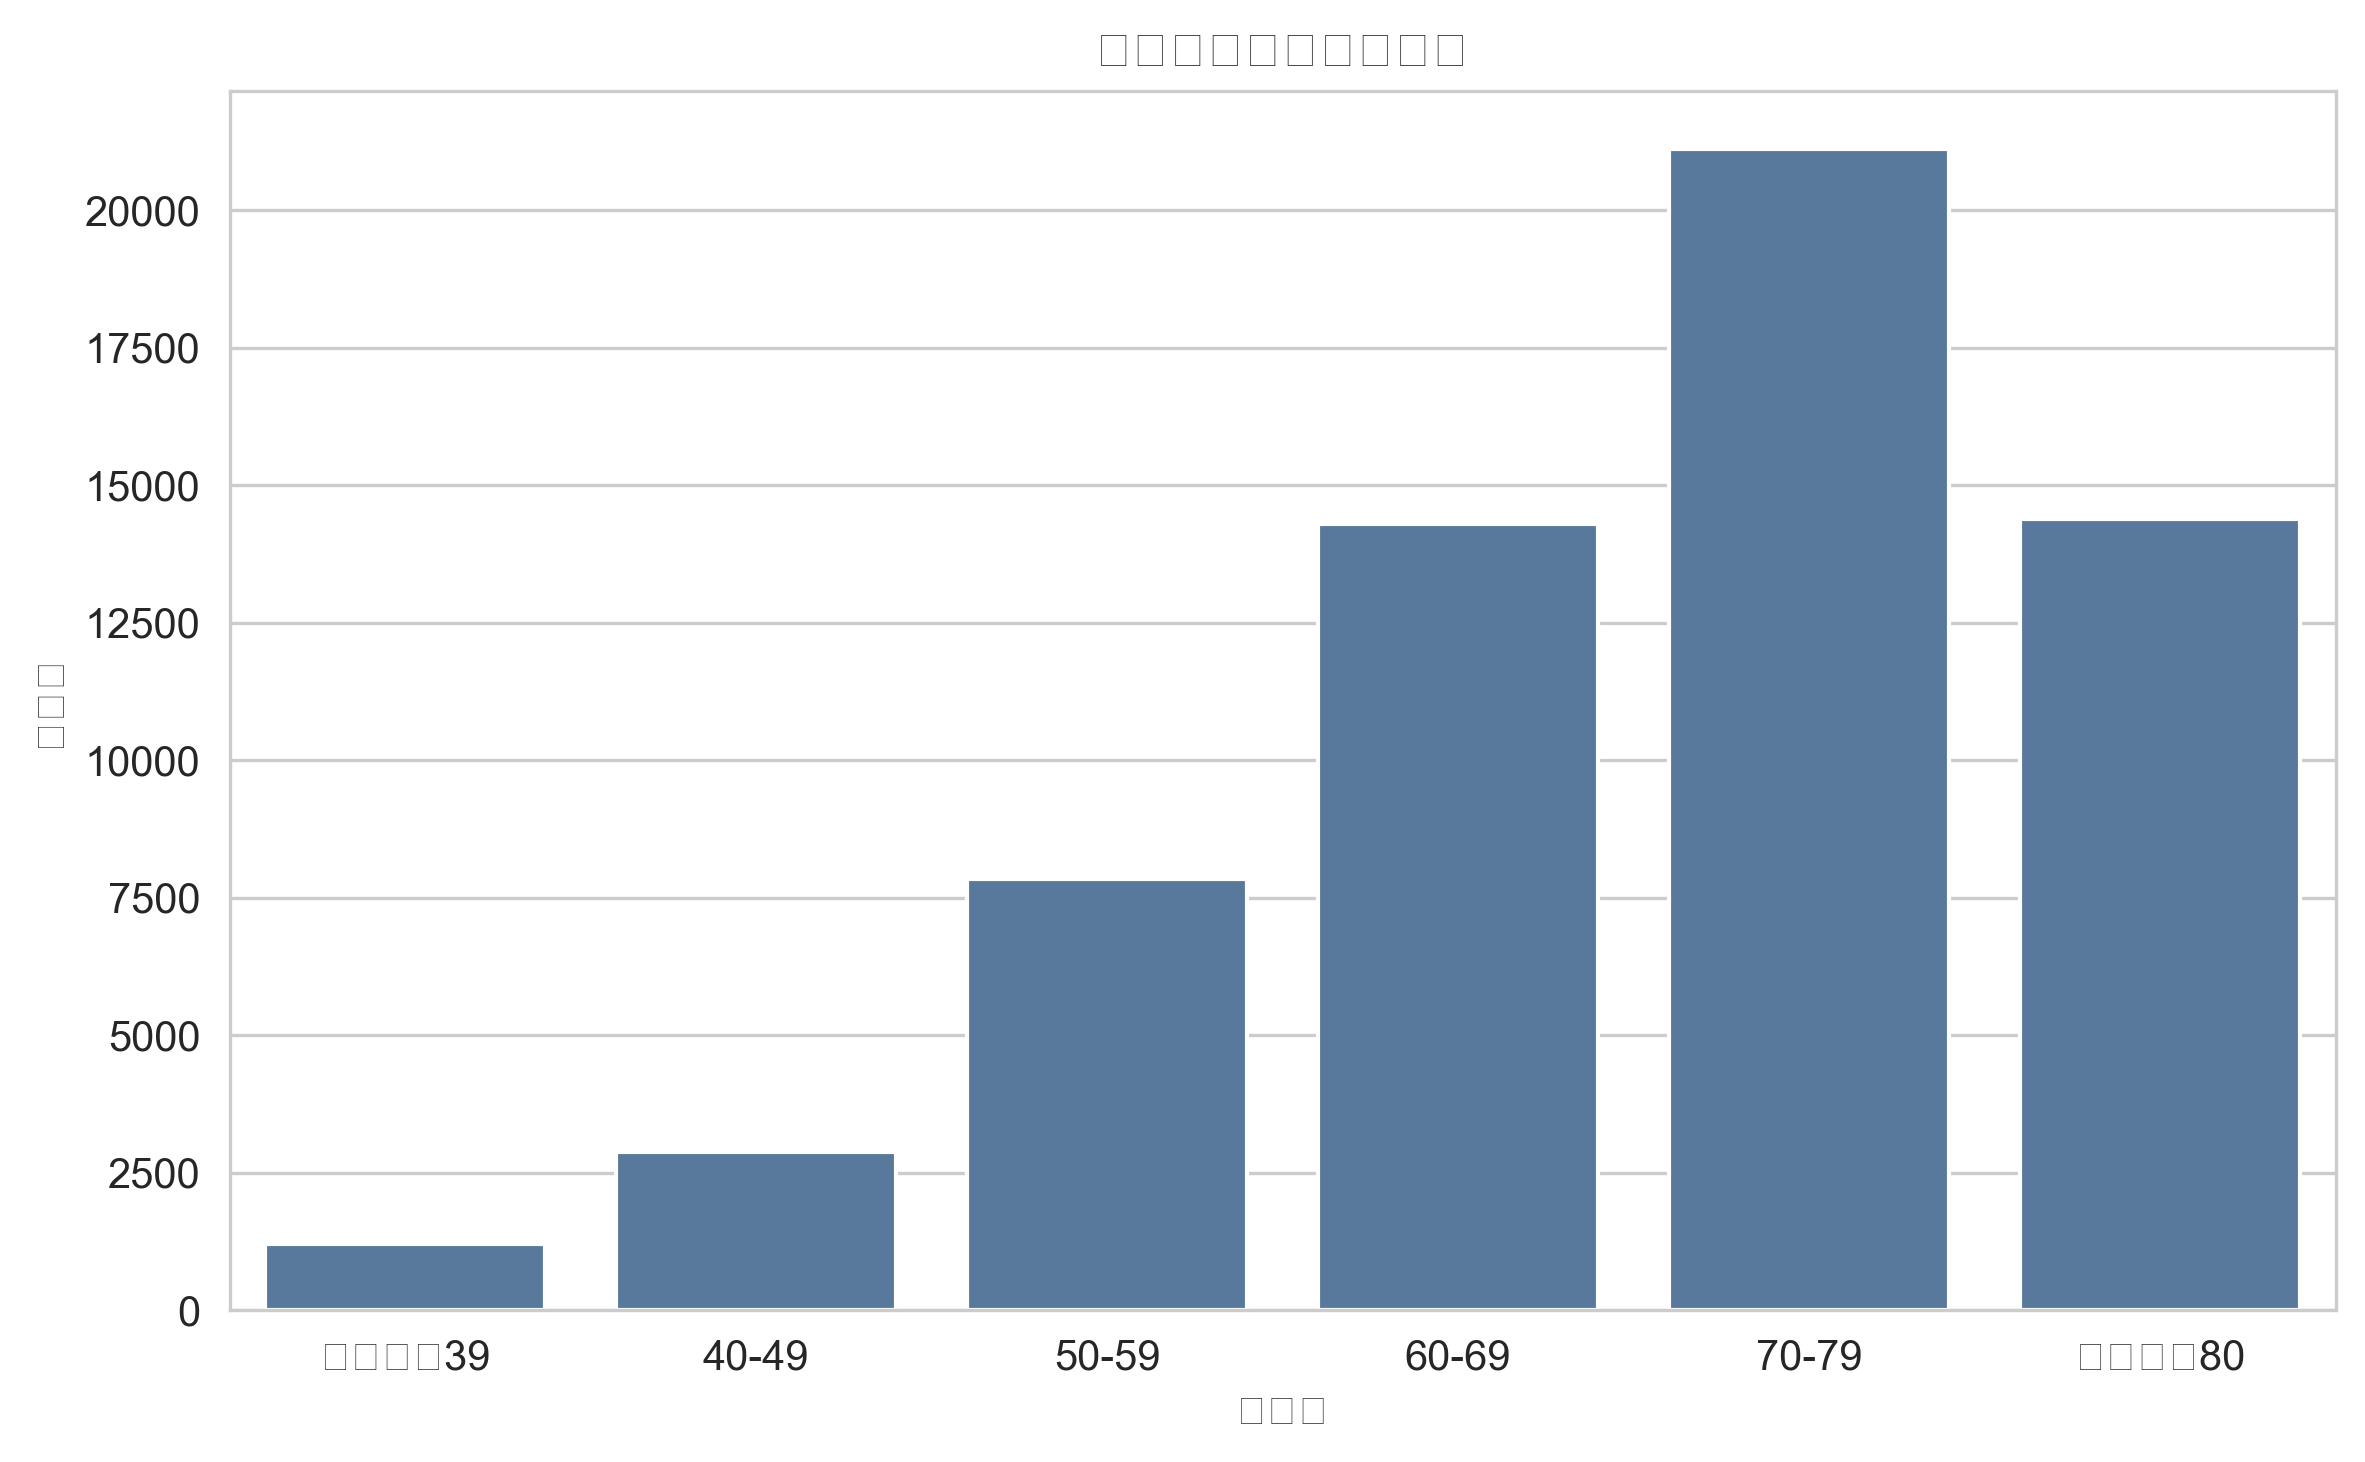
\includegraphics[width=.78\textwidth]{../quest1/figures/q1_age_distribution.png}
\caption{脑卒中病例年龄组分布}
\end{figure}
\begin{figure}[H]\centering
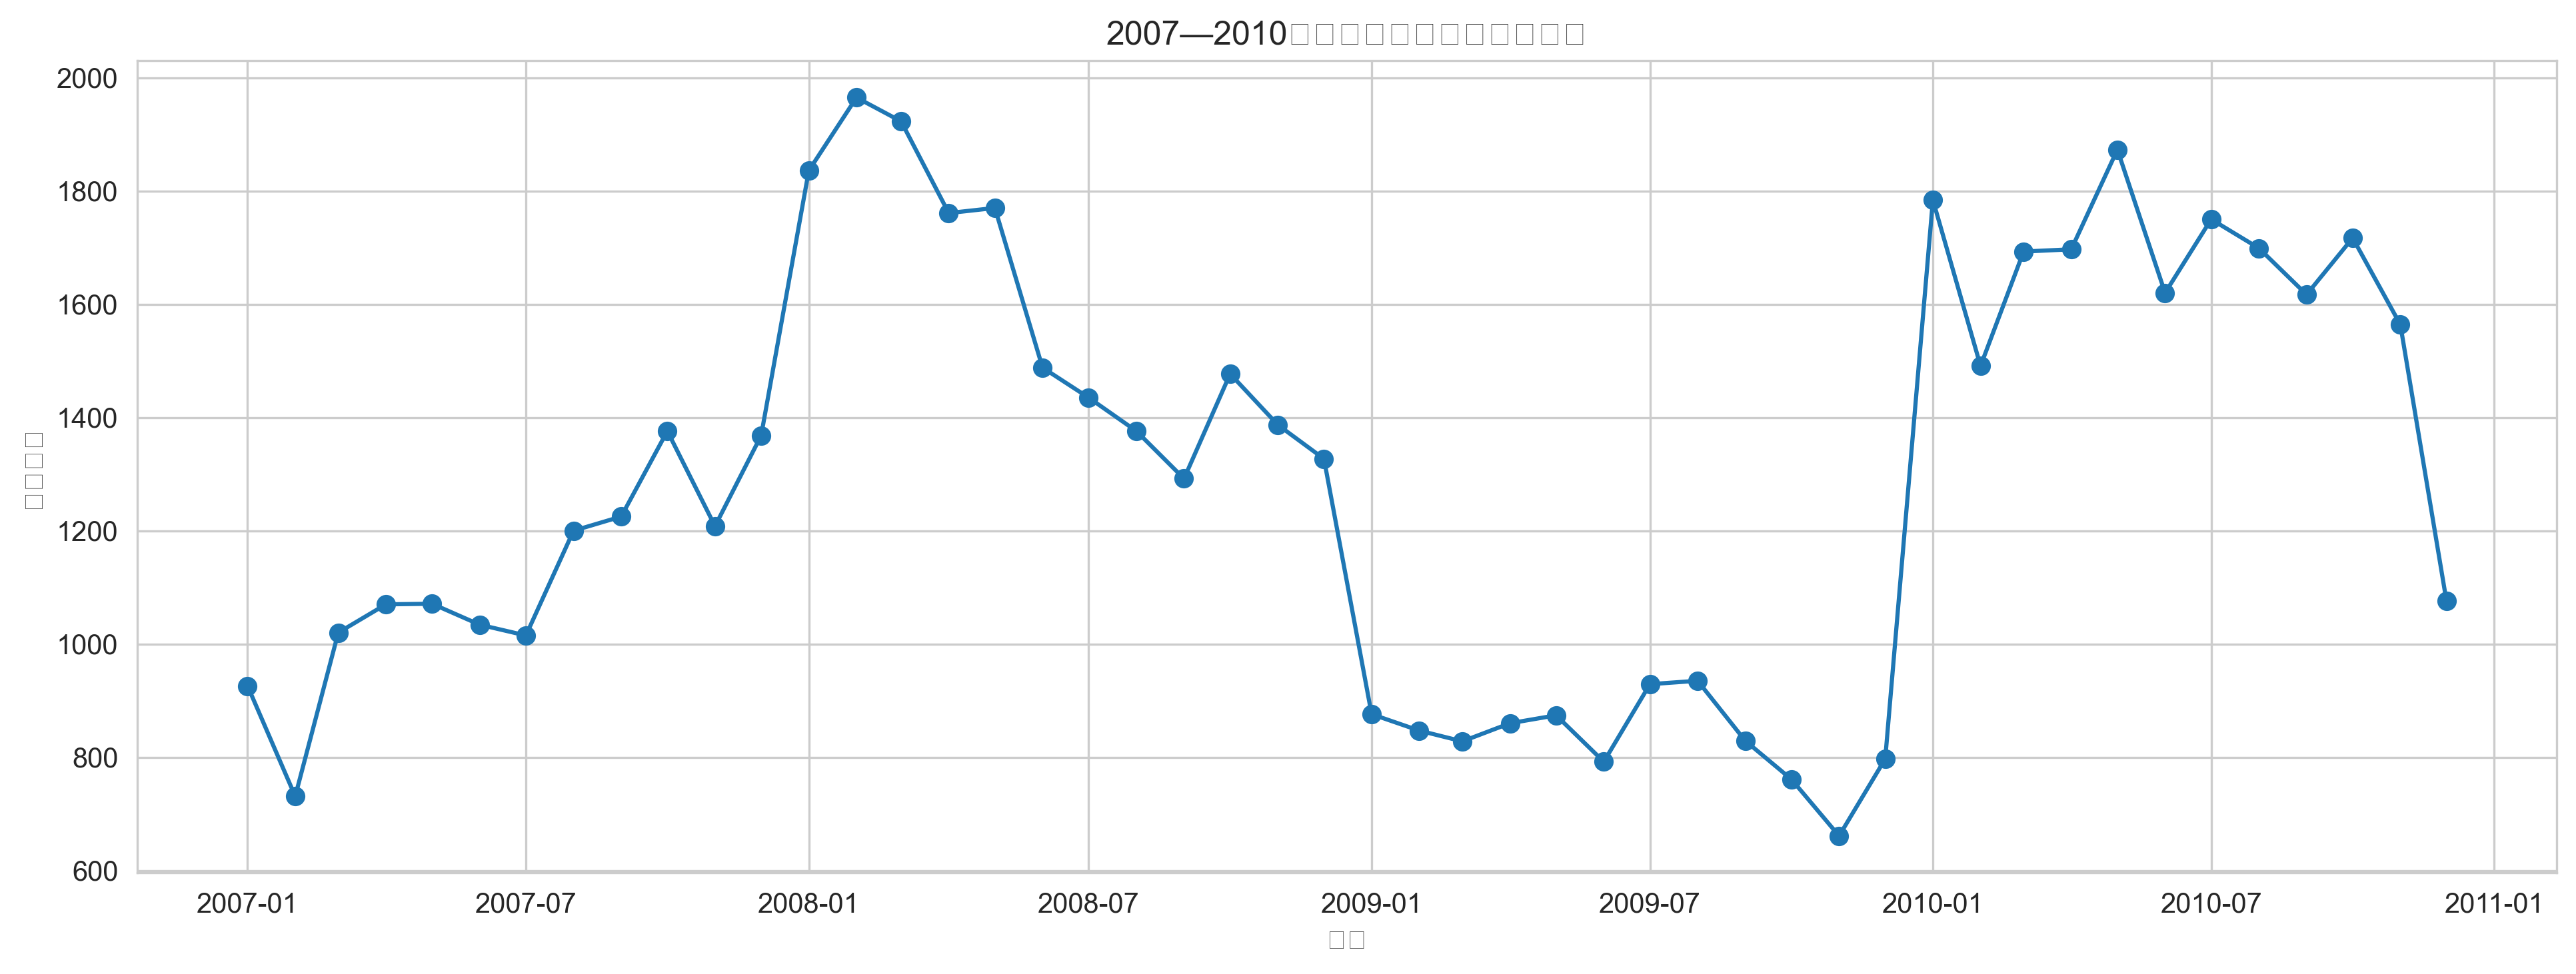
\includegraphics[width=.82\textwidth]{../quest1/figures/q1_monthly_trend.png}
\caption{2007--2010年月度脑卒中发病人数变化}
\end{figure}
月度趋势图显示，病例数并非均匀分布，而是在不同月份存在起伏。最高发月份为2008-02，病例数为1965例。该现象提示仅做全年总体统计不足以支持资源配置，卫生部门还应关注季节性和短期气象诱发的叠加效应。

\subsection{问题二：发病率与气象因素关系模型}
\subsubsection{Baseline模型}
为了检验气象变量是否提供额外解释力，先建立不含气象变量的baseline模型。设$Y_t$为第$t$天病例数，假设
\begin{equation}
Y_t\sim \mathrm{Poisson}(\mu_t),\quad \log(\mu_t)=\beta_0+\beta_1 t+\beta_2\sin\left(\frac{2\pi d_t}{365.25}\right)+\beta_3\cos\left(\frac{2\pi d_t}{365.25}\right),
\end{equation}
其中$d_t$为一年中的第几天。该模型只刻画长期趋势和年周期，是判断气象变量增益的对照组。

\subsubsection{分布滞后Poisson气象回归}
主模型在baseline基础上加入气温、气压、相对湿度及短期滞后项：
\begin{equation}
\log(\mu_t)=\beta_0+\beta_1 t+\beta_2\sin\left(\frac{2\pi d_t}{365.25}\right)+\beta_3\cos\left(\frac{2\pi d_t}{365.25}\right)+\sum_j \gamma_j Z_{j,t},
\end{equation}
其中$Z_{j,t}$包括当天平均气温、平均气压、平均相对湿度、温差、气压差以及1日、3日、7日滞后均值。所有连续变量标准化后进入模型，因此系数$\gamma_j$表示对应变量增加一个标准差时对$\log(\mu_t)$的影响，相对危险度为
\begin{equation}
RR_j=\exp(\gamma_j).
\end{equation}
当$RR_j>1$时，该变量升高与发病数上升相关；当$RR_j<1$时，该变量升高与发病数下降相关。

\subsubsection{模型对比结果}
训练集取2007年1月至2010年6月，测试集取2010年7月至2010年12月。表\ref{tab:modelcomp}给出模型对比。主模型AIC比baseline降低451.3，伪$R^2$由0.050提高到0.121；测试MAE由15.513变为16.412，说明加入气象变量改善了整体拟合解释，但在测试期对尖峰日的点预测并未优于简单季节模型。因此本文将该模型用于风险解释和分级预警辅助，而不是宣称其可精确预测每一天病例数。
\begin{table}[H]\centering\caption{Baseline与主模型对比}\label{tab:modelcomp}
\begin{tabular}{lllll}
\toprule
模型 & AIC & 测试MAE & 测试RMSE & 伪R2 \\
\midrule
Baseline：趋势+年度周期 & 13134.014 & 15.513 & 18.436 & 0.050 \\
主模型：Poisson分布滞后气象回归 & 12682.753 & 16.412 & 19.377 & 0.121 \\
\bottomrule
\end{tabular}
\end{table}

\begin{figure}[H]\centering
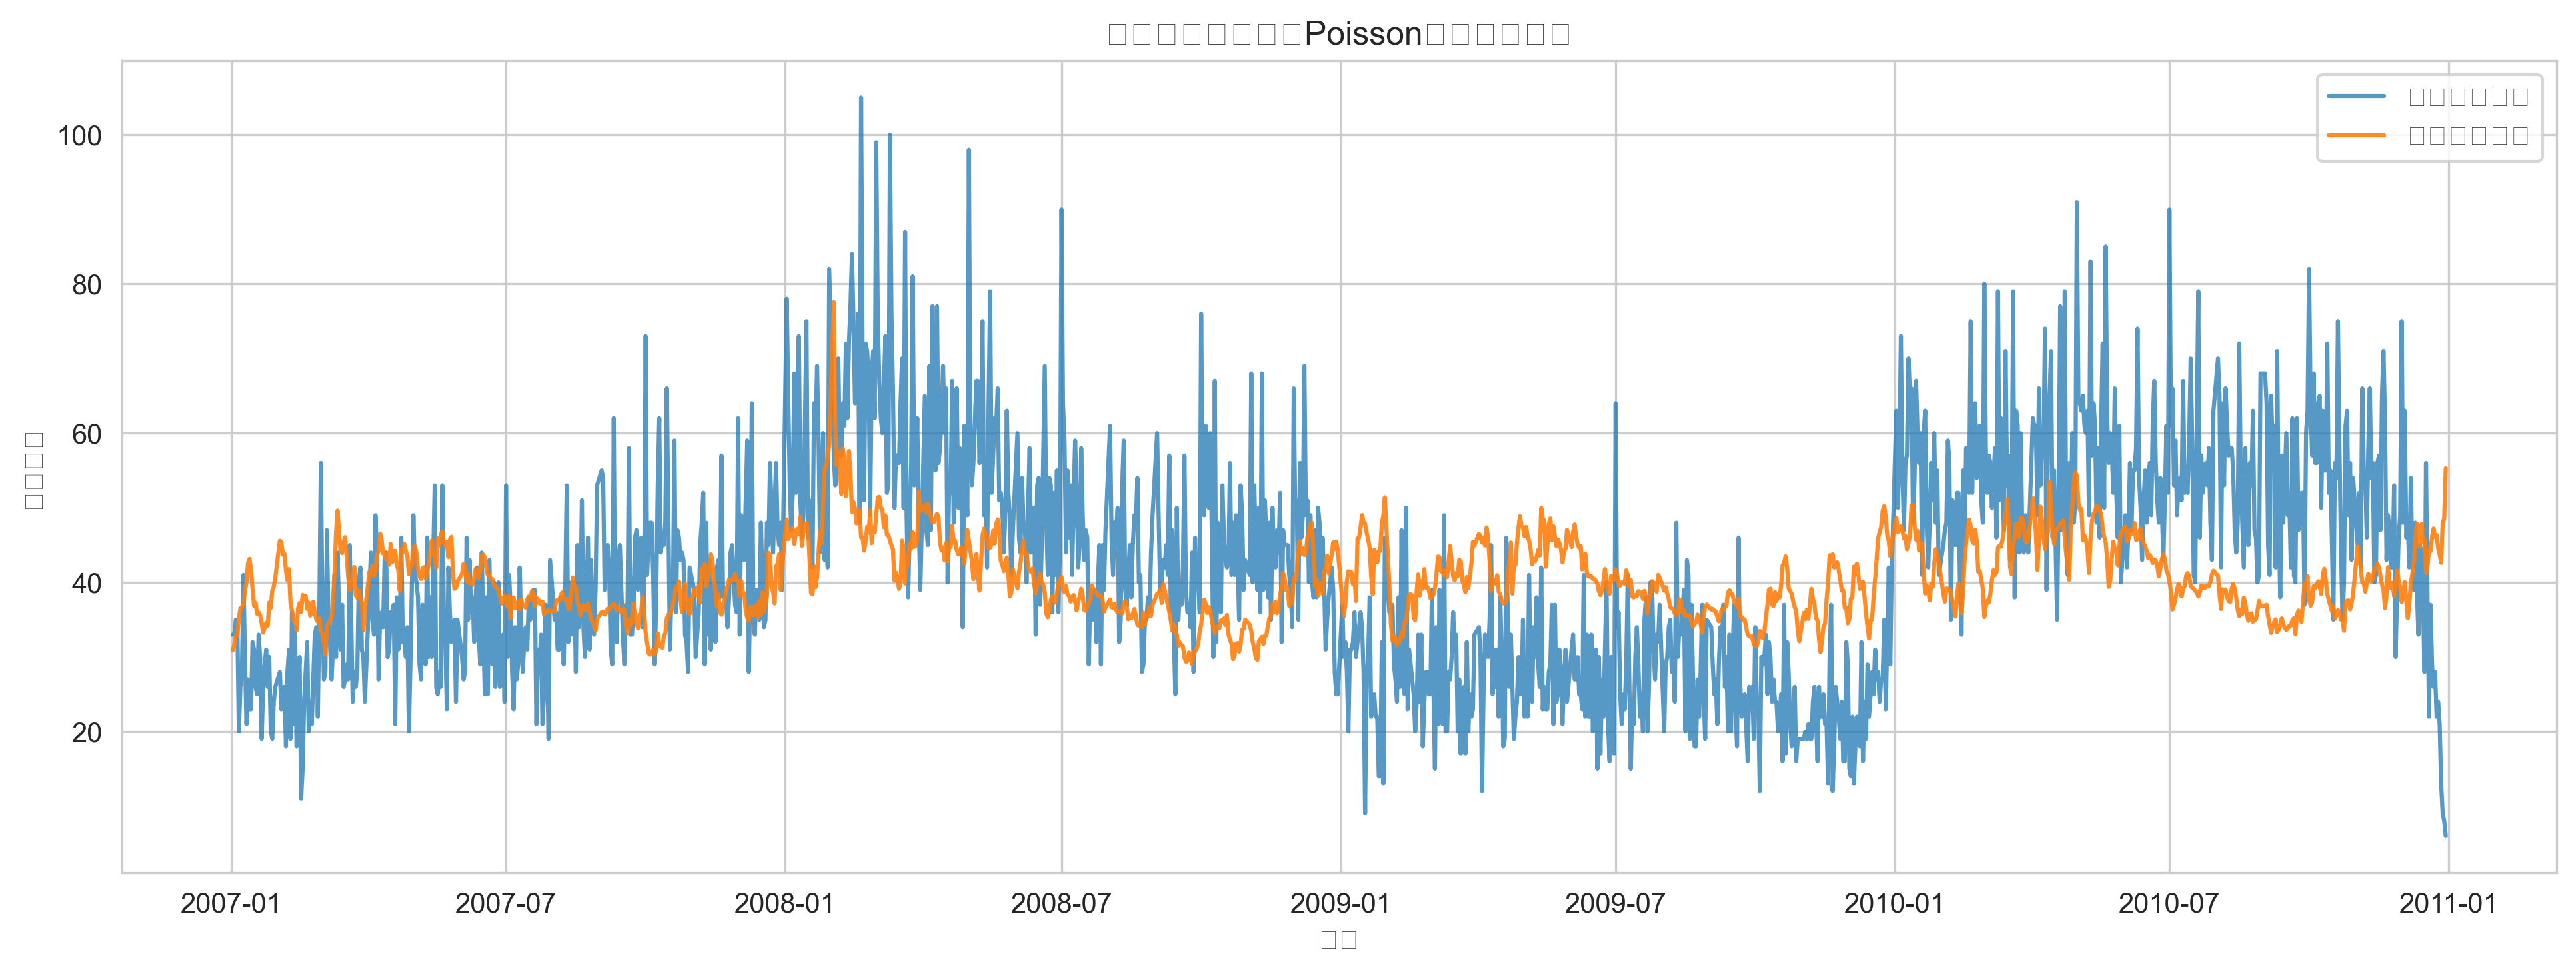
\includegraphics[width=.92\textwidth]{../quest2/figures/q2_daily_fit.png}
\caption{日发病数与Poisson气象模型拟合值}
\end{figure}
图中实际日发病数存在尖峰波动，Poisson模型拟合值更平滑，能捕捉长期趋势和季节水平，但对个别突发高峰仍有低估。这符合医院病例日计数数据的特点：气象因素可以解释部分系统性波动，但个体基础疾病、节假日就医行为、医院报告延迟等未观测因素仍会造成剩余误差。

\subsubsection{变量关系与系数解释}
表\ref{tab:corr}给出日发病数与气象变量的Spearman相关系数。相关分析只反映单变量关系，不能排除季节和趋势混杂，因此本文以Poisson多变量模型作为主结论来源。
\begin{table}[H]\centering\caption{日发病数与气象变量的Spearman相关性}\label{tab:corr}
\begin{tabular}{lll}
\toprule
变量 & 相关系数 & P值 \\
\midrule
Aver RH & -0.0850 & 0.0014 \\
Min RH & -0.0389 & 0.1450 \\
temp\_range & 0.0330 & 0.2163 \\
High pres & 0.0094 & 0.7260 \\
pres\_range & 0.0081 & 0.7603 \\
Aver pres & 0.0076 & 0.7747 \\
Low temp & -0.0068 & 0.7994 \\
Low pres & 0.0056 & 0.8330 \\
Aver temp & -0.0035 & 0.8957 \\
High temp & 0.0001 & 0.9960 \\
\bottomrule
\end{tabular}
\end{table}

主模型部分关键气象变量系数见表\ref{tab:coef}。由于变量已标准化，系数可直接比较方向和相对强度。若某变量$RR$大于1，表示在其他变量和季节趋势控制不变时，该气象变量升高一个标准差会使期望日发病数按$RR$倍变化。需要注意的是，温度、气压、湿度之间存在季节相关性，个别系数不能简单解释为严格因果效应，应结合整体预测改进和敏感性分析共同判断。
\begin{table}[H]\centering\caption{主模型关键气象变量系数与相对危险度}\label{tab:coef}
\begin{tabular}{llll}
\toprule
变量 & 系数 & P值 & 相对危险度RR \\
\midrule
Aver temp & 0.0296 & 0.6570 & 1.0300 \\
Aver temp\_lag3 & -0.0151 & 0.8976 & 0.9850 \\
Aver pres & 0.0371 & 0.3264 & 1.0378 \\
Aver pres\_lag3 & -0.0615 & 0.3962 & 0.9404 \\
Aver RH & -0.0318 & 0.0108 & 0.9687 \\
Aver RH\_lag3 & 0.0223 & 0.3230 & 1.0226 \\
temp\_range & -0.0157 & 0.2214 & 0.9844 \\
pres\_range & 0.0106 & 0.3791 & 1.0106 \\
\bottomrule
\end{tabular}
\end{table}

\begin{figure}[H]\centering
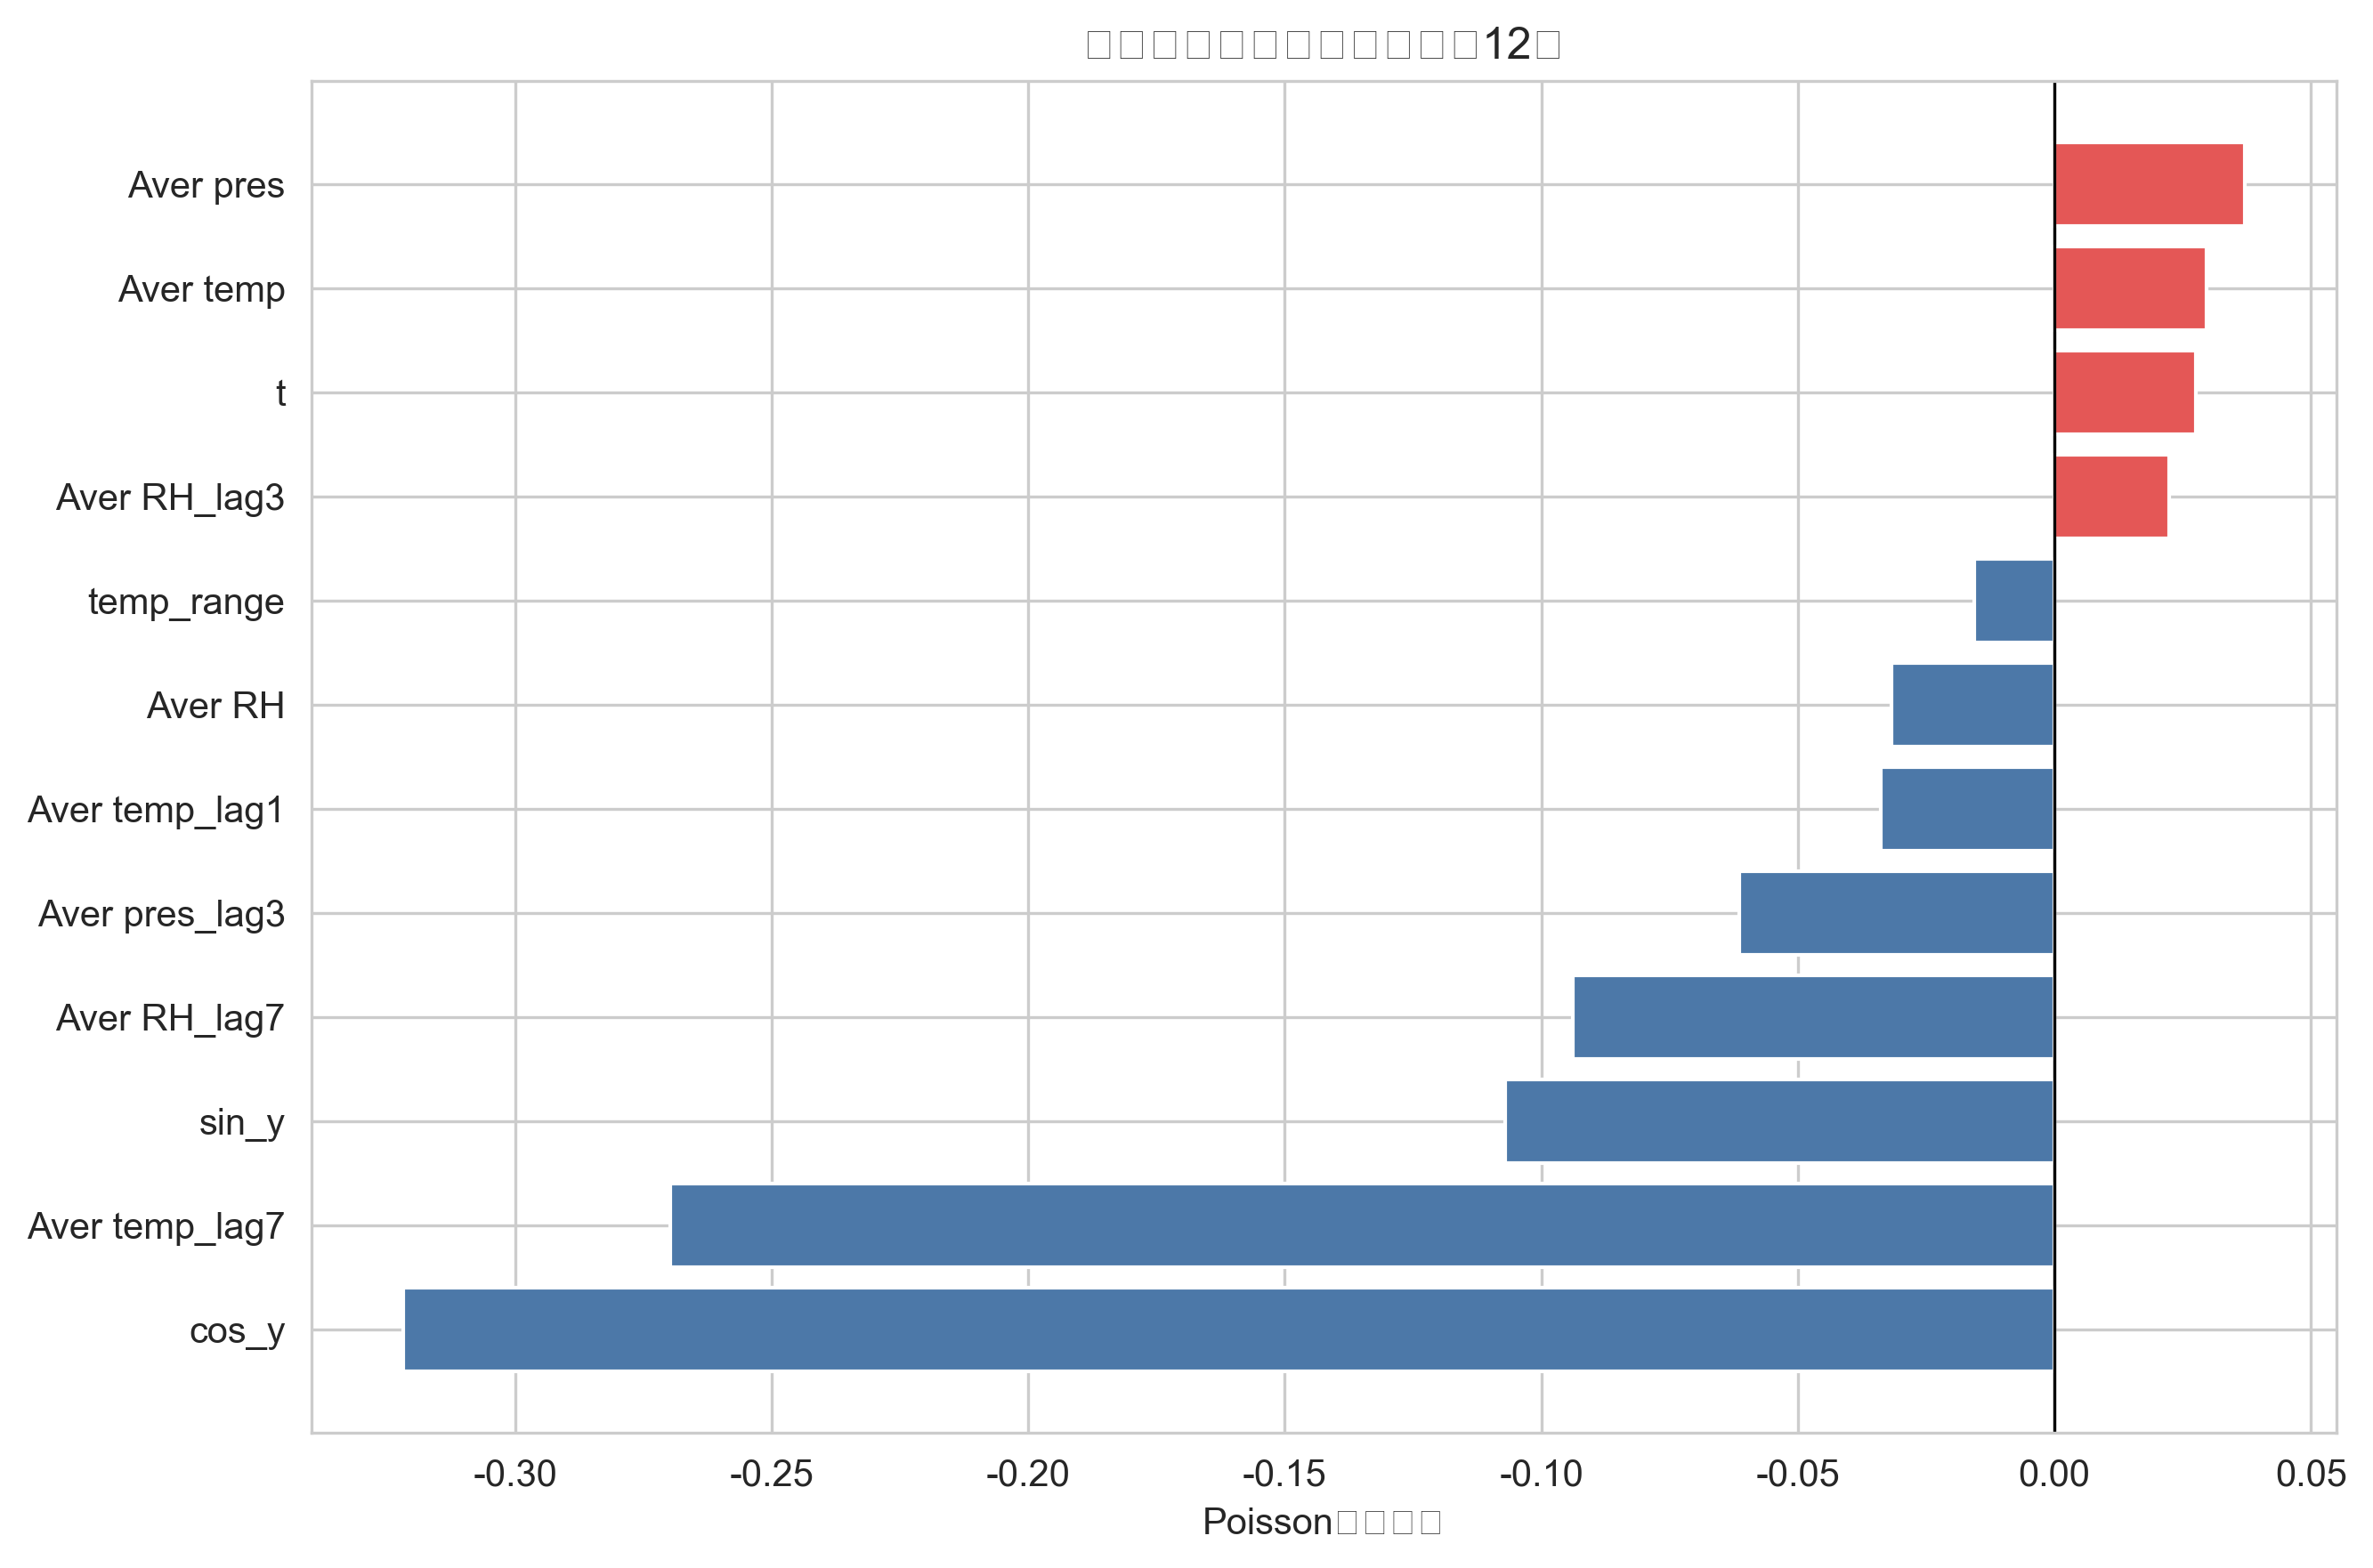
\includegraphics[width=.82\textwidth]{../quest2/figures/q2_top_coefficients.png}
\caption{主模型标准化系数绝对值前12项}
\end{figure}
该图展示了对模型影响较大的标准化变量。正系数表示风险随变量升高而上升，负系数表示风险随变量升高而下降。由于加入了多种滞后项，某些当天变量和滞后变量可能方向不同，这反映短期气象变化过程并非单调作用。例如连续多日均值与当天异常变化可能代表不同环境情景，因此预警时不宜只看单日某一个指标。

\subsection{问题三：高危人群预警与干预模型}
\subsubsection{高危人群指标体系}
结合医学文献和公共卫生实践，脑卒中高危因素主要包括高龄、男性、既往卒中或短暂性脑缺血发作、高血压、糖尿病、血脂异常、房颤、吸烟、肥胖和缺乏运动等。本题病例数据只提供年龄、性别、职业和发病时间，缺少慢病史，因此本文将题目数据能够支持的因素作为基础分层，将慢病史等关键指标作为实际应用中必须补充采集的字段。表\ref{tab:demo}列出了数据支持的主要预警依据。
\begin{table}[H]\centering\caption{预警方案的数据依据}\label{tab:demo}
\begin{tabular}{lll}
\toprule
指标 & 关键发现 & 预警含义 \\
\midrule
年龄 & 病例年龄均值69.8岁，中位数72.0岁，60岁及以上占80.5\% & 年龄是最稳定的人群分层指标，60岁以上应作为重点筛查对象。 \\
性别 & 男性33358例，占53.9\% & 男性比例较高，应结合吸烟、饮酒、职业暴露强化干预。 \\
职业 & 农民占比最高，为48.0\% & 职业分布受城市人口结构影响，但可用于社区随访名单排序。 \\
气象 & 主模型相对baseline AIC降低451.3，测试MAE变化5.8\% & 气象变量能改善整体拟合解释，但样本外尖峰预测仍有误差，适合作为辅助预警而非唯一判据。 \\
\bottomrule
\end{tabular}
\end{table}

\subsubsection{综合风险评分模型}
定义综合风险分$S$为
\begin{equation}
S=S_{age}+S_{sex}+S_{occ}+S_{chronic}+S_{meteo},
\end{equation}
其中$S_{age}$由年龄分层给出，$S_{sex}$和$S_{occ}$为人口学修正分，$S_{chronic}$由高血压、糖尿病、既往卒中等慢病史给出，$S_{meteo}$由问题二模型预测的日风险分位给出。若只使用题目数据，则可先计算群体层面的$S_{meteo}$；若接入社区健康档案，则可进一步形成个体化预警。
\begin{table}[H]\centering\caption{年龄基础风险分规则}\label{tab:agescore}
\begin{tabular}{lll}
\toprule
特征 & 分值 & 干预建议 \\
\midrule
年龄小于50岁 & 0 & 常规健康教育，关注血压血脂。 \\
50-59岁 & 15 & 每年至少一次卒中危险因素筛查。 \\
60-69岁 & 30 & 加强血压、血糖、血脂管理，气象风险日减少户外暴露。 \\
70-79岁 & 45 & 建立家庭/社区随访，寒冷或气压剧烈变化时主动提醒。 \\
80岁及以上 & 55 & 列为重点高危人群，异常天气日提前备药并保持就医通道。 \\
\bottomrule
\end{tabular}
\end{table}

\begin{figure}[H]\centering
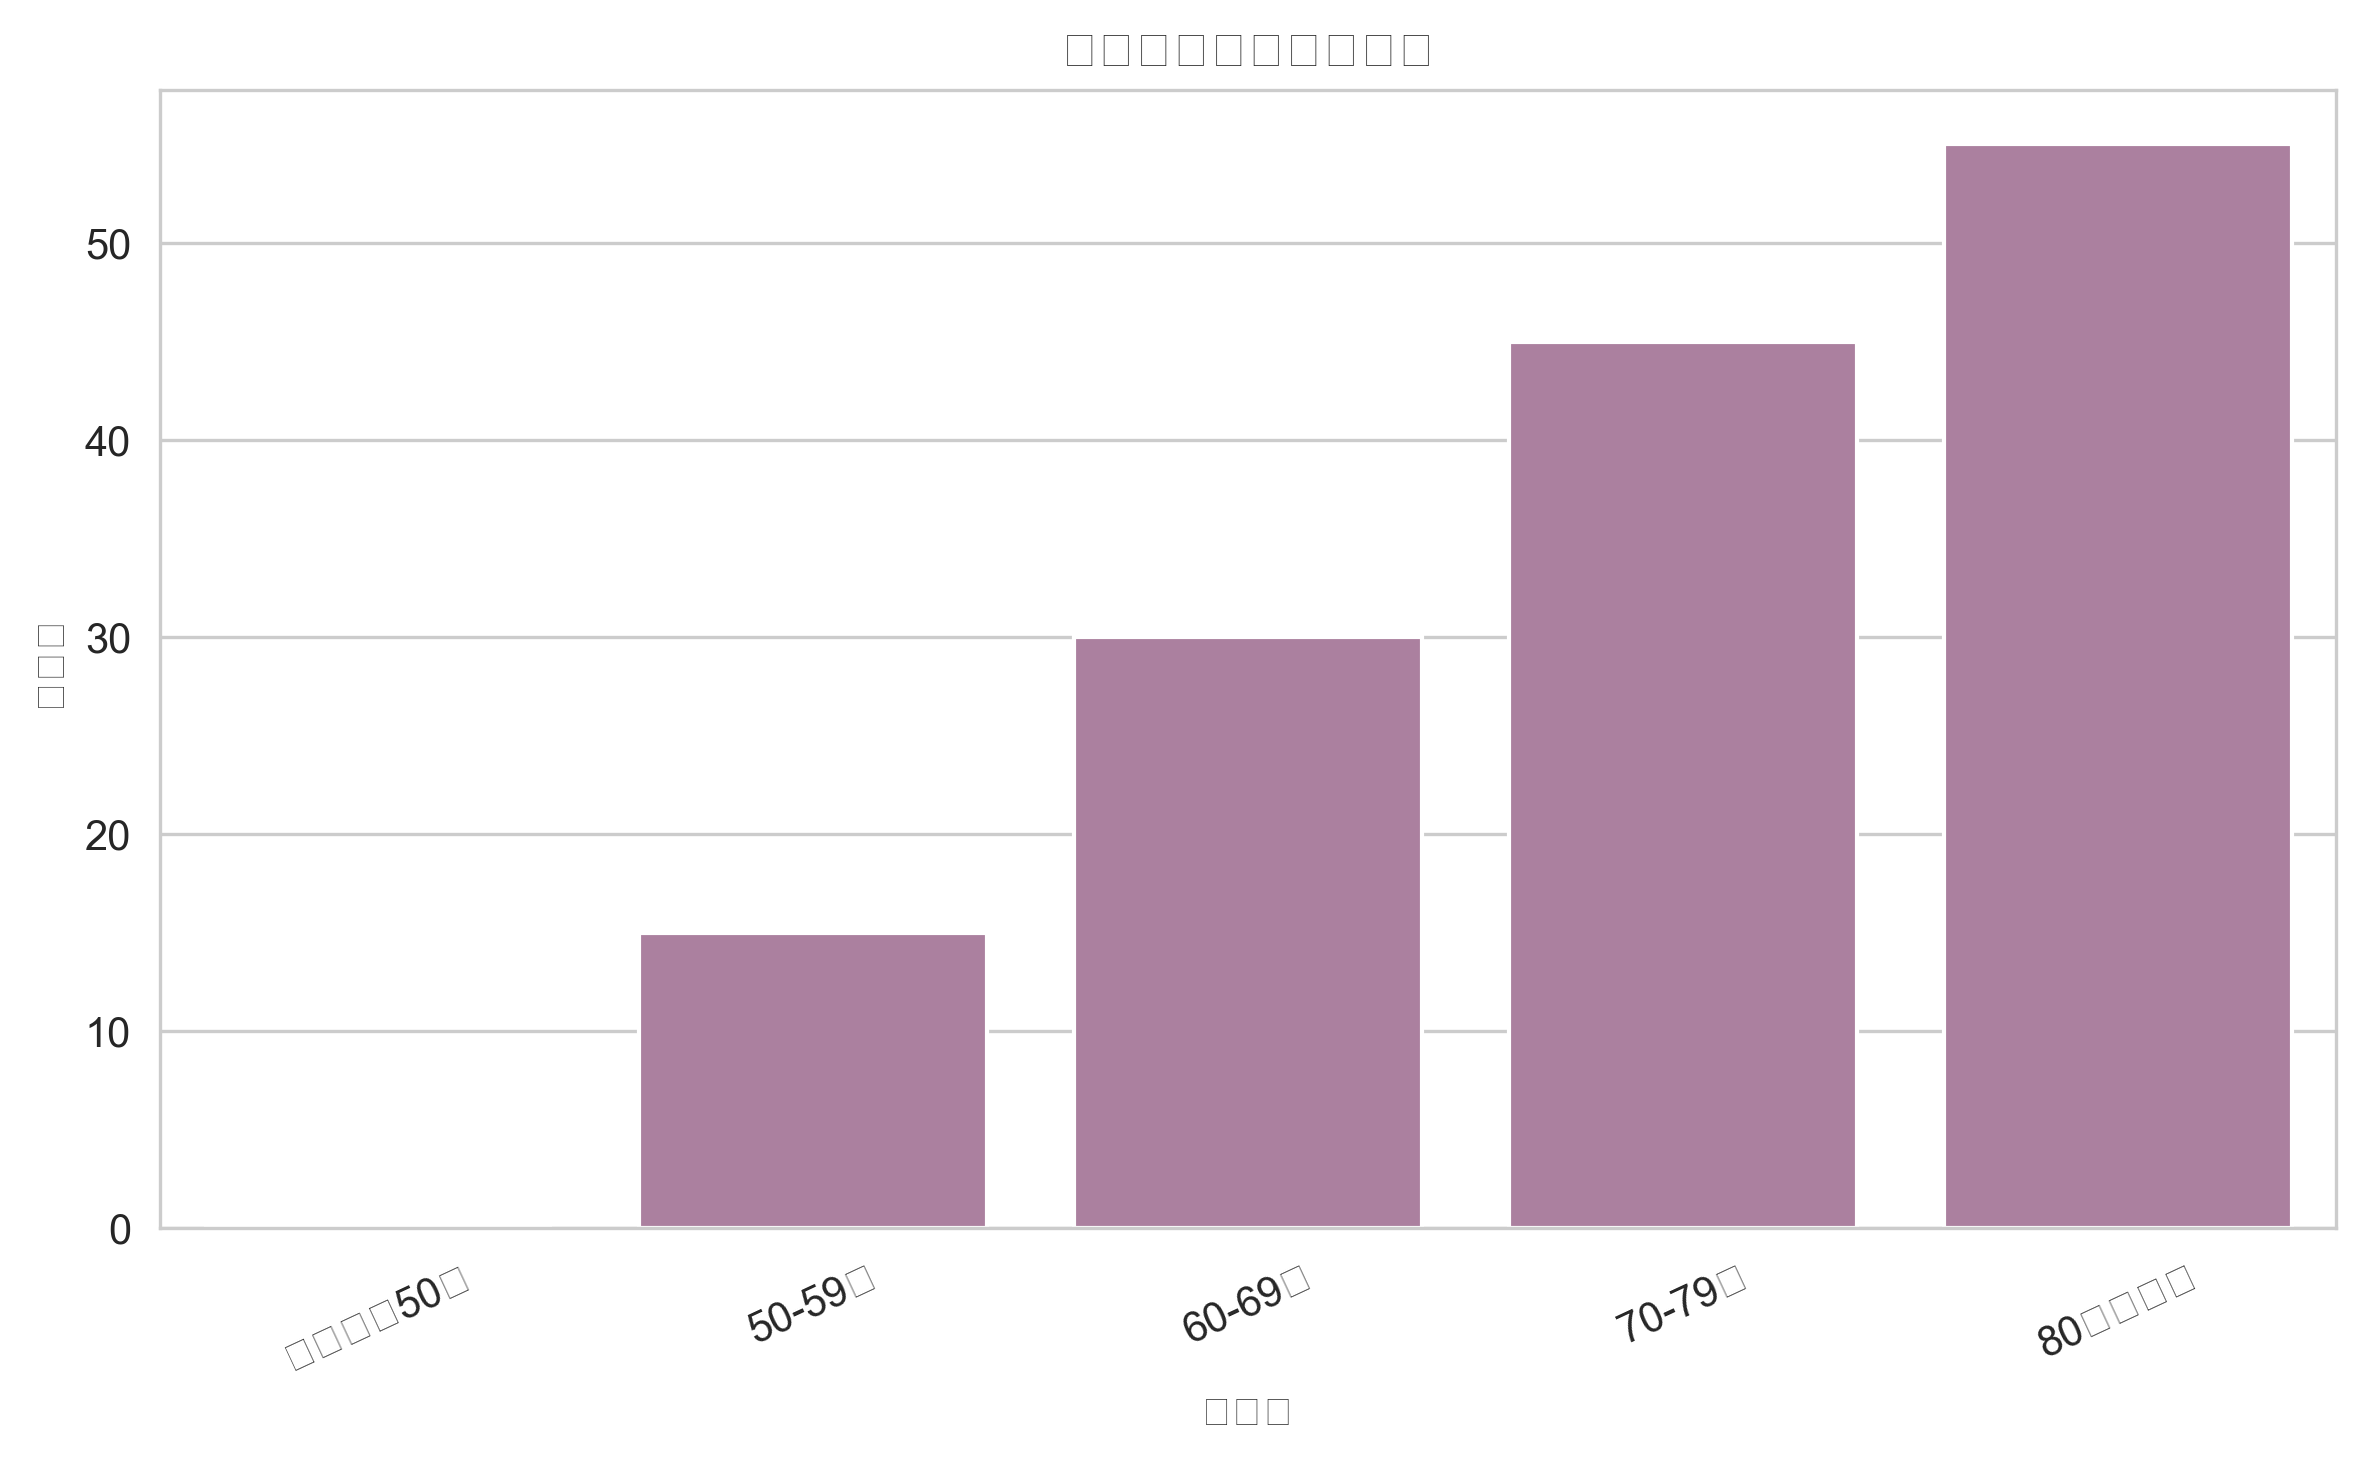
\includegraphics[width=.72\textwidth]{../quest3/figures/q3_age_risk_score.png}
\caption{年龄分层预警基础分值}
\end{figure}
年龄基础分随年龄上升而增加，是因为问题一显示病例高度集中于中老年人群，且医学上年龄增长会显著增加动脉粥样硬化、血管弹性下降和合并慢病概率。该分值不是诊断结论，而是用于社区筛查排序和预警消息优先级划分。

\subsubsection{四级气象—人群联动预警}
预警等级按$S$和模型预测风险分位共同确定。建议阈值为：50分以上蓝色，70分以上黄色，85分以上橙色，95分以上红色；若气象模型预测风险超过历史90\%分位，即使个体基础分较低，也应提高群体健康提醒强度。表\ref{tab:rules}给出四级预警规则。
\begin{table}[H]\centering\caption{四级预警触发条件与建议措施}\label{tab:rules}
\begin{tabular}{lll}
\toprule
预警等级 & 触发条件 & 建议措施 \\
\midrule
蓝色 & 模型预测日发病风险处于历史50\%—75\%分位，或单个气象关键因子进入轻度不利区间 & 社区卫生服务中心发布健康提醒，高血压/糖尿病人群自测血压。 \\
黄色 & 模型预测风险处于75\%—90\%分位，或气温、气压、湿度中两个因子同时不利 & 对60岁以上慢病人群短信/电话提醒，减少剧烈活动，保证室内温湿度。 \\
橙色 & 模型预测风险处于90\%—97.5\%分位，且近期温度/气压有明显波动 & 社区医生主动随访重点名单，医院适当增加急诊和神经内科值班资源。 \\
红色 & 模型预测风险超过97.5\%分位或连续多日橙色风险 & 卫生行政部门启动短期应急预案，媒体发布防护提示，医疗机构预留床位和溶栓绿色通道。 \\
\bottomrule
\end{tabular}
\end{table}

\subsubsection{分对象干预方案}
预警的价值在于提前干预而非事后解释。本文将干预对象分为健康/亚健康人群、60岁以上慢病人群、既往卒中或TIA人群、医疗机构和卫生行政部门五类。对应措施见表\ref{tab:inter}。
\begin{table}[H]\centering\caption{分对象干预方案}\label{tab:inter}
\begin{tabular}{ll}
\toprule
对象 & 措施 \\
\midrule
健康/亚健康人群 & 建立生活方式干预：控烟限酒、低盐饮食、规律运动、监测血压；在蓝色及以上气象风险日减少突然冷热暴露。 \\
60岁以上或有高血压/糖尿病/高血脂者 & 纳入社区重点随访；黄色预警起每日血压监测，出现口角歪斜、肢体无力、言语不清立即就医。 \\
既往卒中/TIA或多危险因素叠加者 & 橙色预警起主动电话随访，检查服药依从性，必要时提前门诊复诊或调整治疗计划。 \\
医疗机构 & 依据预测风险调整急诊、神经内科、影像检查和床位资源；连续高风险日增加卒中绿色通道保障。 \\
卫生行政部门 & 把气象预警嵌入公共卫生信息平台，形成“气象—社区—医院”联动机制并定期评估误报/漏报。 \\
\bottomrule
\end{tabular}
\end{table}

\section{模型检验、对比与稳健性分析}
\subsection{Baseline对比}
Baseline只含趋势与年度周期，主模型在相同训练/测试切分下加入气象变量。AIC降低451.3支持主模型在全样本拟合优度与复杂度权衡上优于baseline；但测试MAE变化为5.8\%，提示2010年下半年存在若干尖峰日，使复杂模型的点预测误差略高。因此本文对模型的定位是“解释气象关联并辅助风险预警”，而非替代临床或公共卫生监测系统的精确日预测。

\subsection{残差诊断}
\begin{figure}[H]\centering
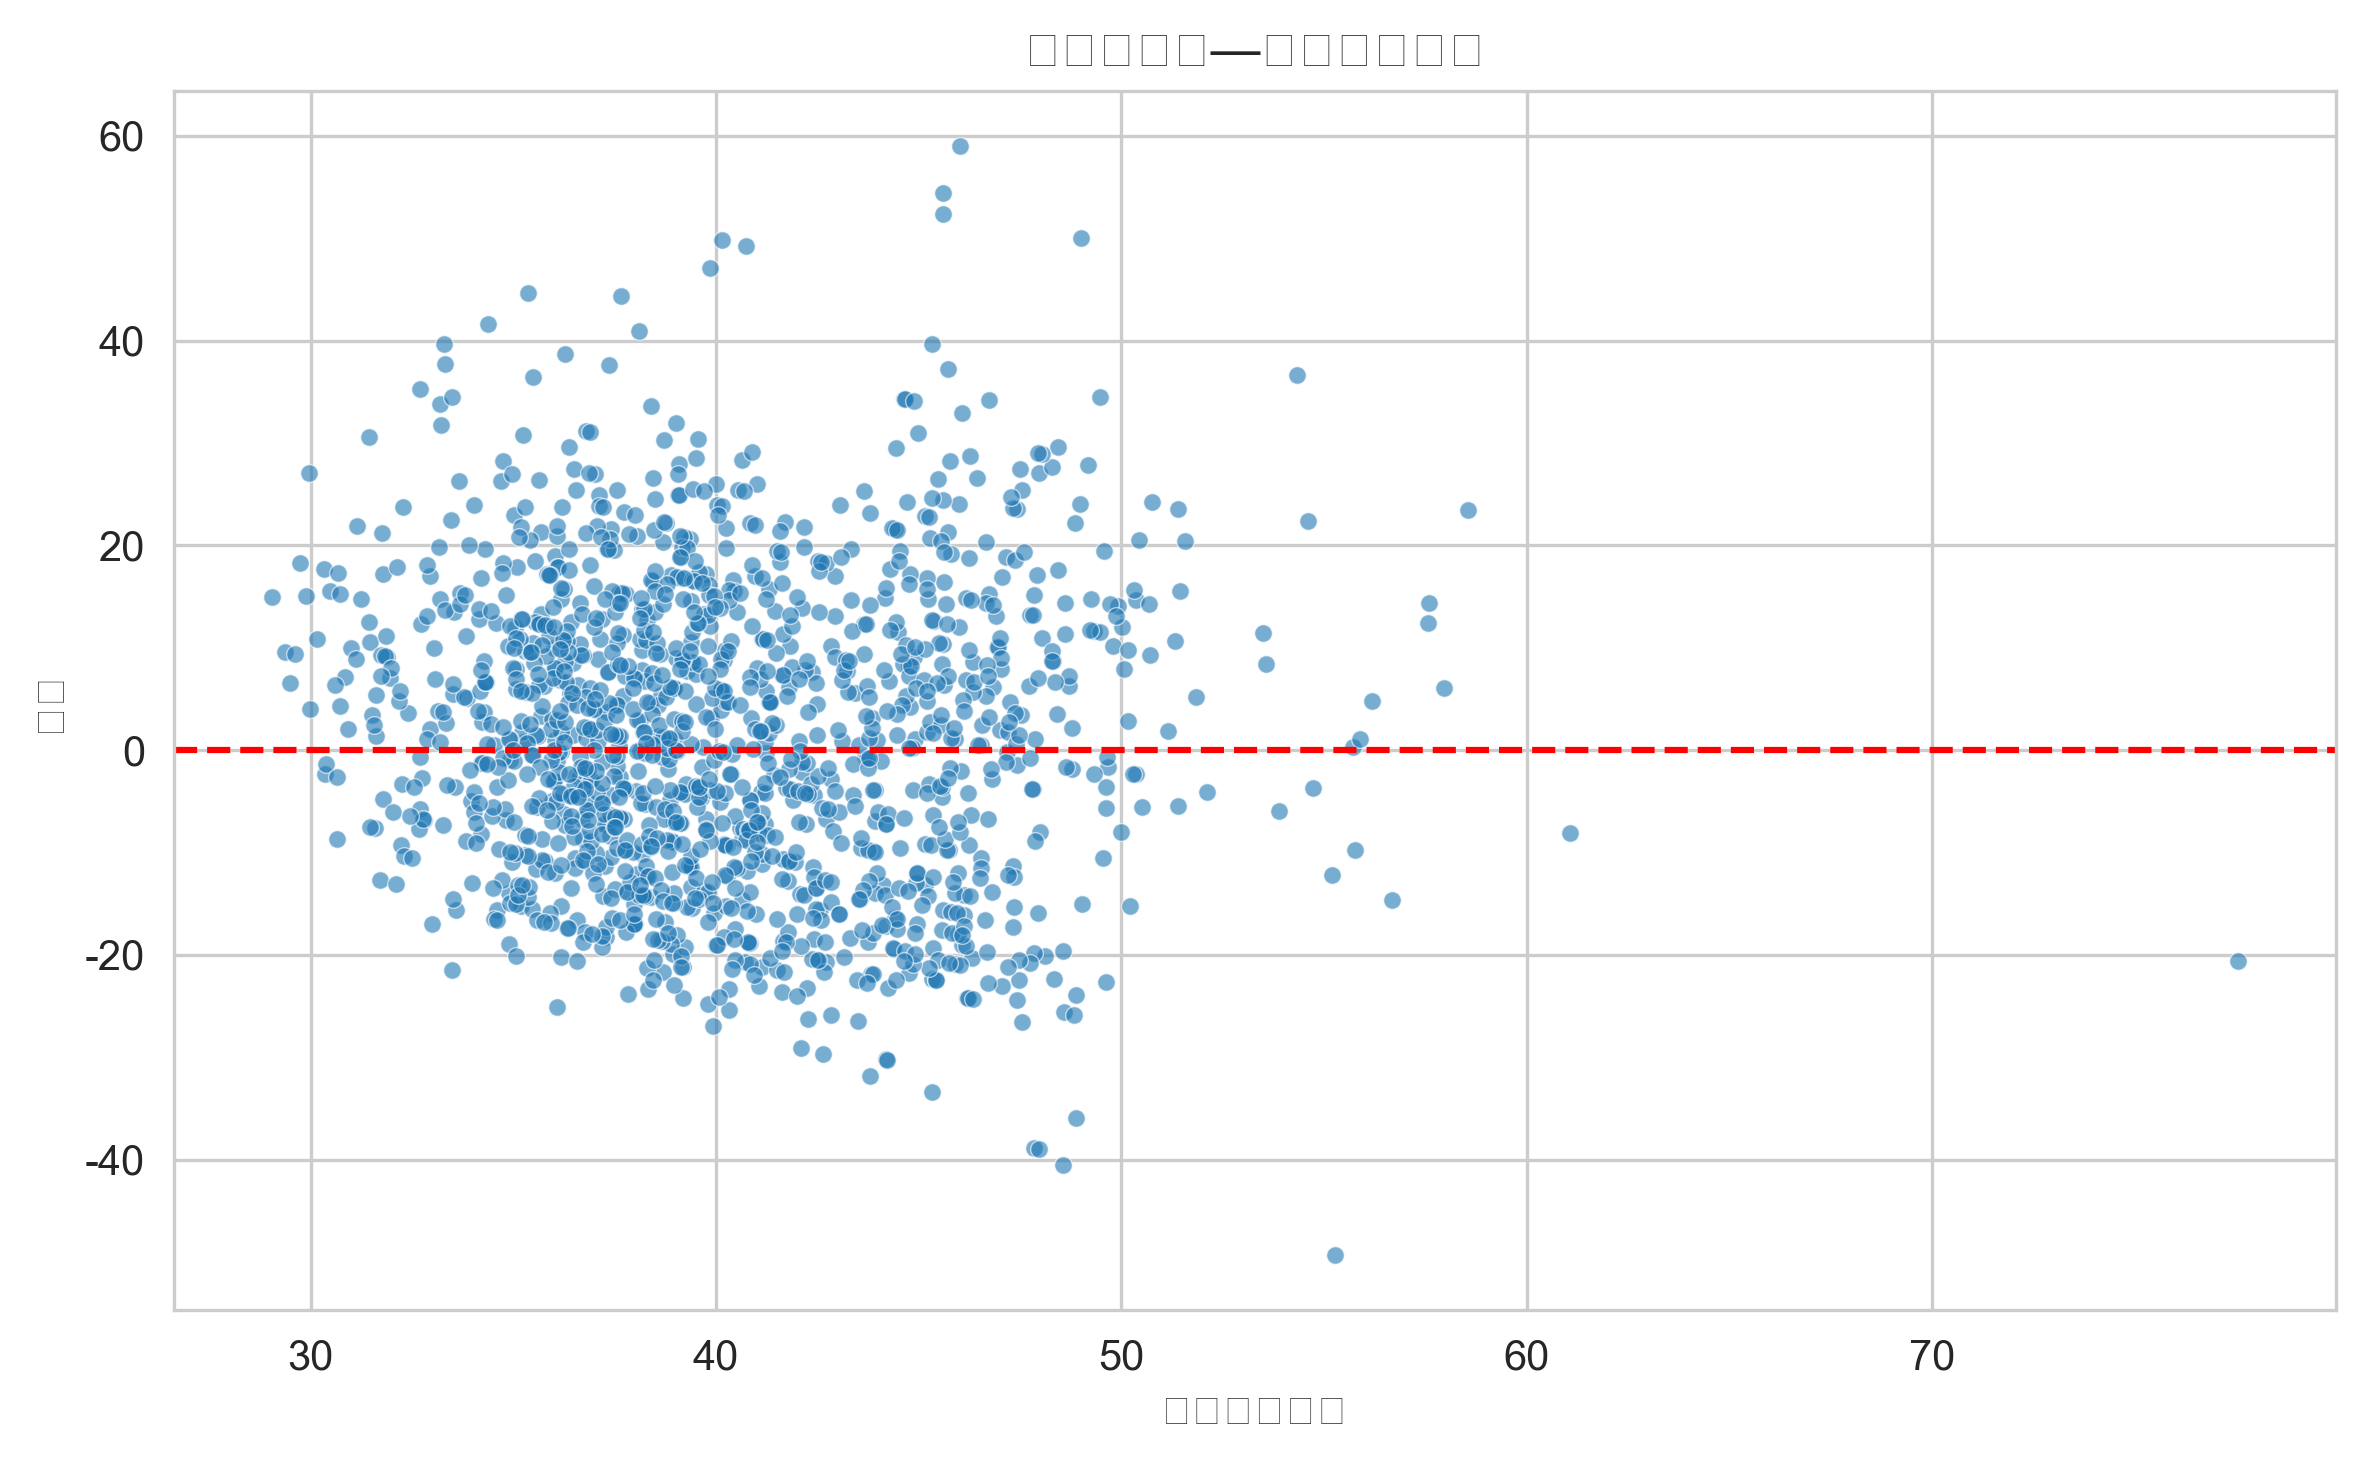
\includegraphics[width=.72\textwidth]{../quest2/figures/q2_residual_diagnostic.png}
\caption{Poisson主模型残差诊断图}
\end{figure}
残差图中大多数点围绕0上下波动，说明模型不存在明显系统性偏移；但在拟合值较高区域仍可见较大正残差，表示个别高发日未被气象变量充分解释。这提示后续改进应加入空气污染、节假日、流感流行、医院报告制度变化和个体慢病史等因素。

\subsection{敏感性分析}
本文对关键气象变量进行正负一个标准差扰动，并用$RR=\exp(\beta)$衡量期望日发病数变化。表\ref{tab:sens}和图展示了敏感性结果。若$RR$偏离1越远，表示模型对该变量越敏感。该分析可用于预警系统解释：当敏感变量进入不利区间时，应提高风险提示等级。
\begin{table}[H]\centering\caption{关键气象变量扰动的相对危险度}\label{tab:sens}
\begin{tabular}{llll}
\toprule
参数 & +1标准差RR & -1标准差RR & 系数 \\
\midrule
Aver pres\_lag3 & 0.9404 & 1.0634 & -0.0615 \\
Aver RH & 0.9687 & 1.0323 & -0.0318 \\
Aver temp\_lag3 & 0.9850 & 1.0152 & -0.0151 \\
Aver RH\_lag3 & 1.0226 & 0.9779 & 0.0223 \\
Aver temp & 1.0300 & 0.9708 & 0.0296 \\
Aver pres & 1.0378 & 0.9636 & 0.0371 \\
\bottomrule
\end{tabular}
\end{table}
\begin{figure}[H]\centering
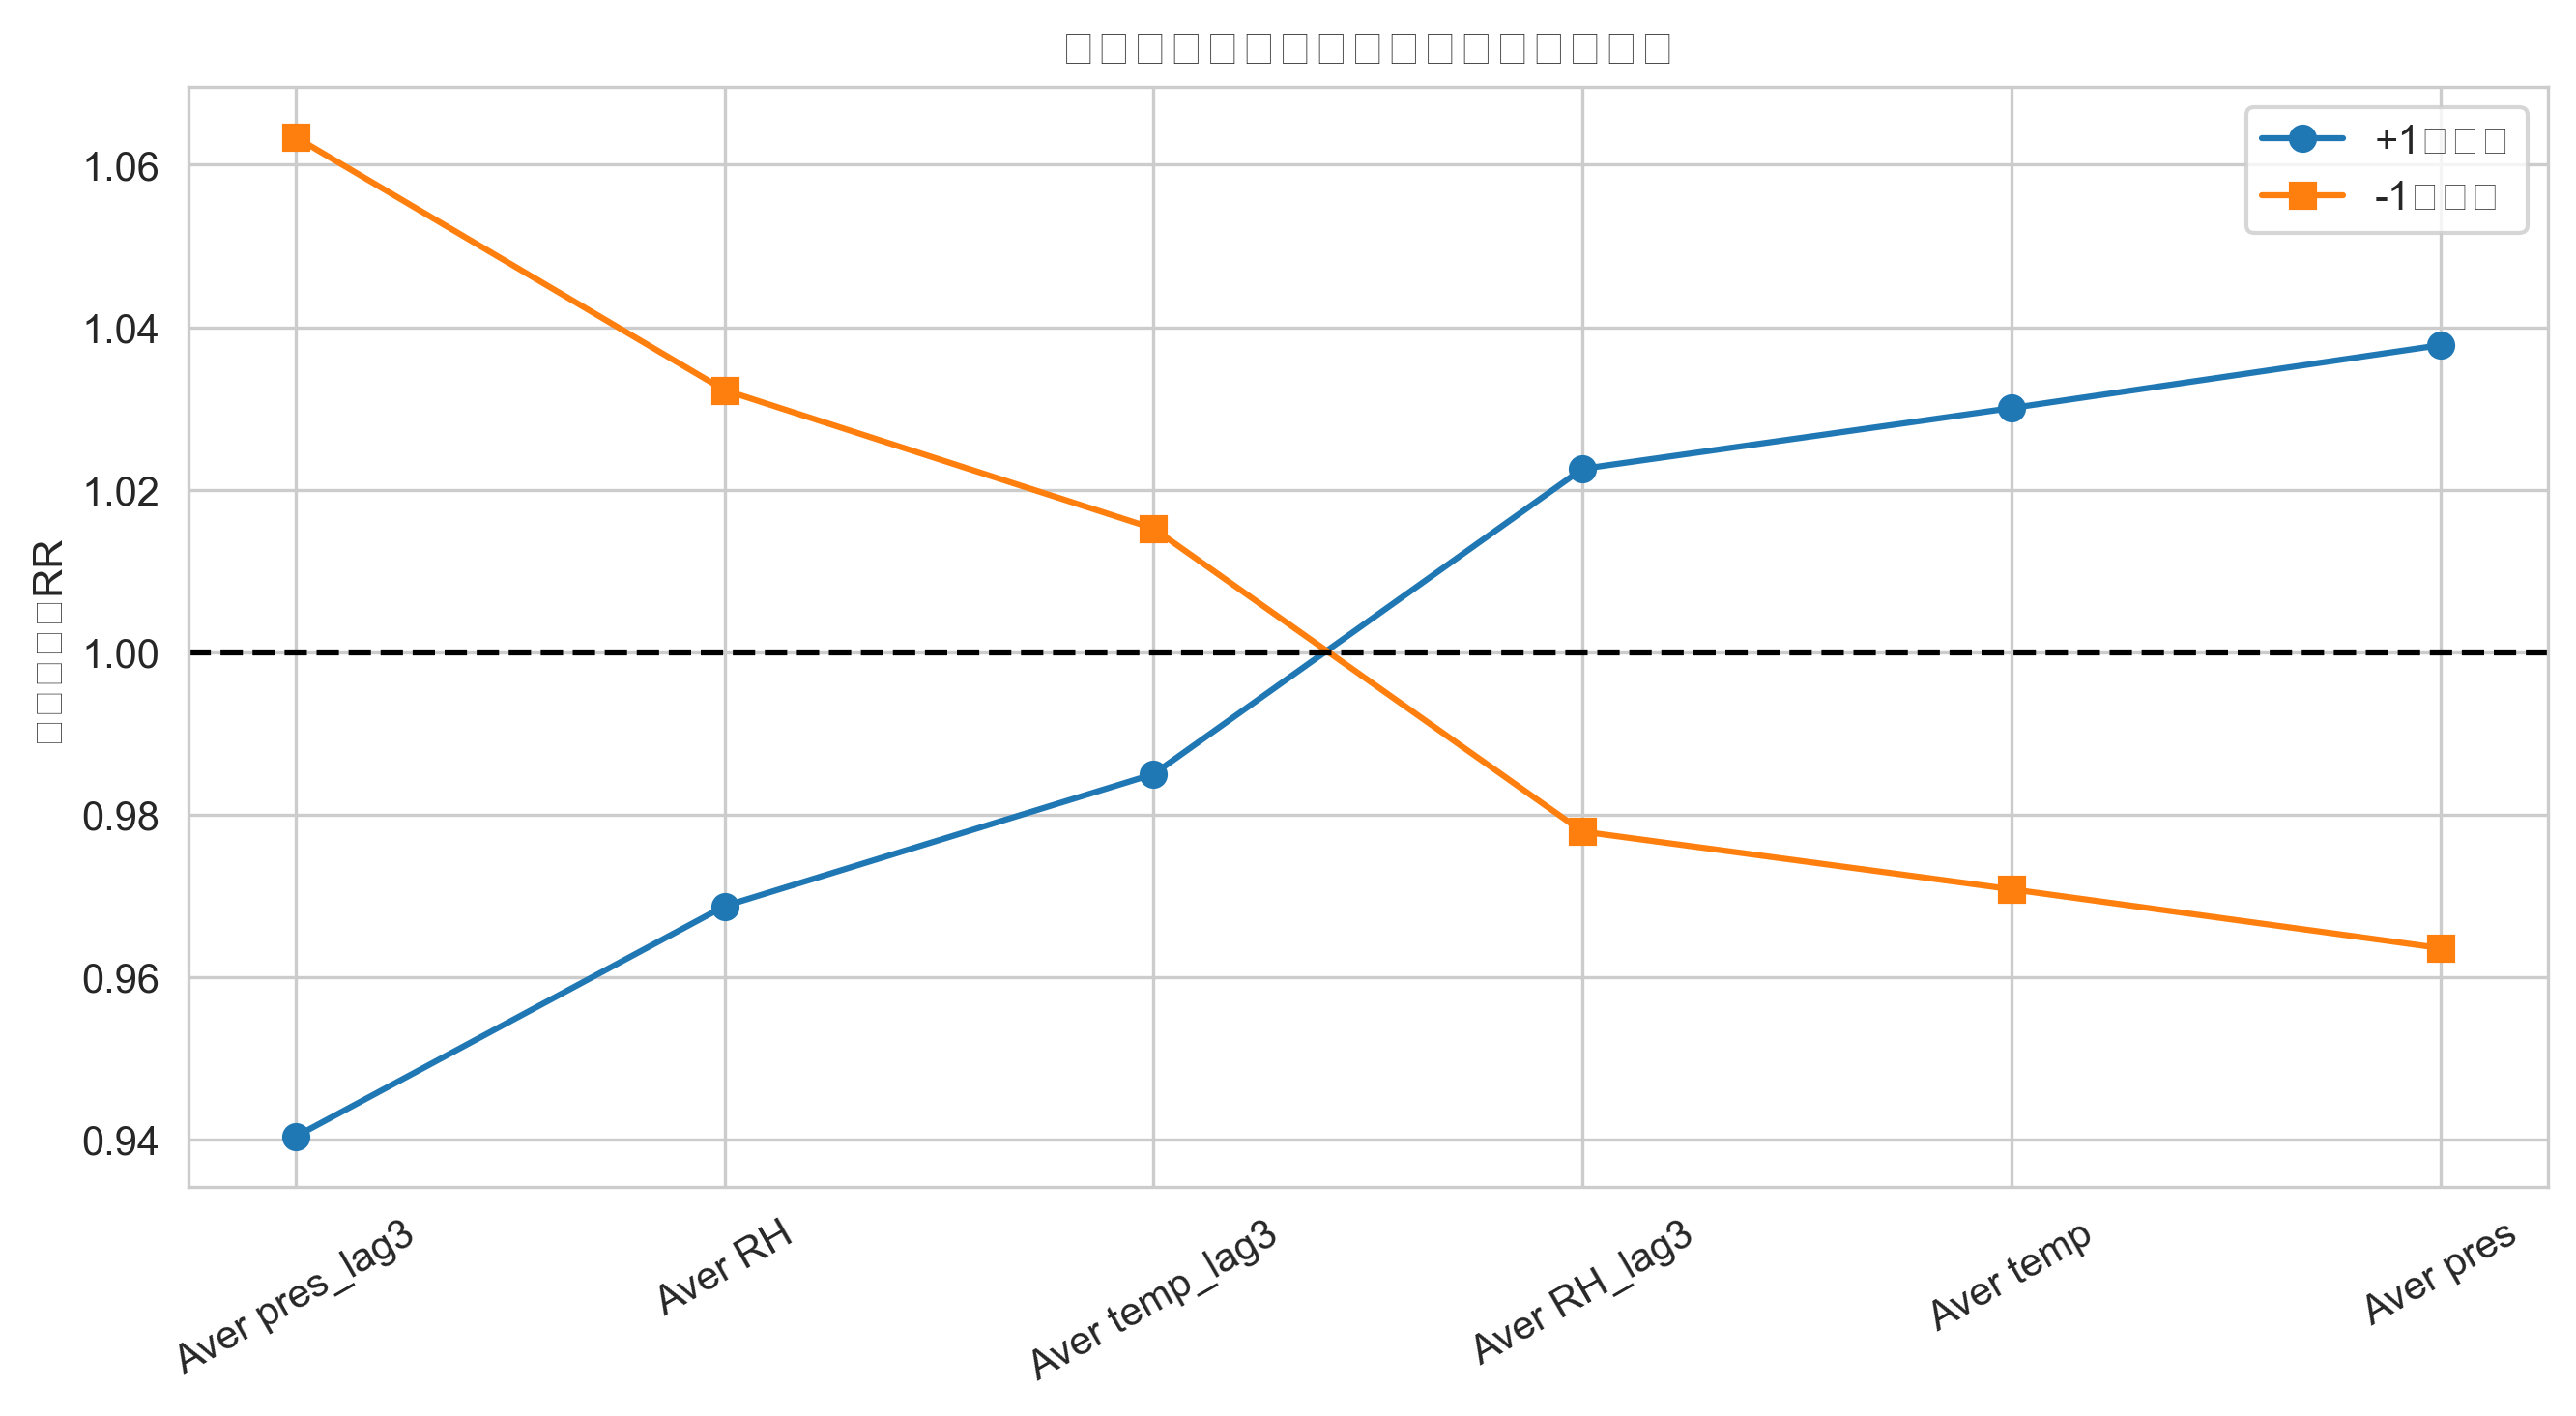
\includegraphics[width=.76\textwidth]{../quest2/figures/q2_sensitivity_rr.png}
\caption{气象变量正负扰动下的相对危险度}
\end{figure}

\section{模型评价、改进与推广}
\subsection{模型优点}
第一，本文模型输出与题目要求直接对应。问题一输出人群统计描述，问题二输出气象因素与日发病数关系，问题三输出预警和干预方案，形成从数据到决策的闭环。第二，问题二采用Poisson计数模型，符合日发病数非负整数的统计性质，并设置baseline对照，避免只给复杂模型而无法判断增量价值。第三，本文将气象变量的当天值和短期滞后值同时纳入，能更好反映环境因素对脑卒中的延迟诱发效应。第四，所有关键数字均由代码生成并写入冻结文件，图表保存到支撑材料目录，具有较好的可复现性。

\subsection{模型局限}
第一，题目未给出城市逐日人口基数和年龄结构，因此本文以日病例数代理发病率变化，无法计算严格意义上的年龄标化发病率。第二，病例数据缺少高血压、糖尿病、吸烟、既往卒中等个体医学信息，第三问的个体预警评分需要在实际部署时接入社区健康档案。第三，气象因素之间存在较强季节相关性，Poisson回归系数可解释为统计关联，但不能直接证明因果关系。第四，模型未包含空气污染、节假日、流感流行和医疗可及性等变量，个别高发日仍可能出现较大残差。

\subsection{改进方向与推广}
后续可从三个方面改进。其一，加入人口基数和分年龄人口结构，建立年龄标化发病率模型；其二，接入个体慢病史和生活方式数据，构建个体级卒中风险评分；其三，引入空气污染、冷空气过程、热浪/寒潮指标和节假日变量，建立更完整的分布滞后非线性模型。本文框架也可推广到心肌梗死、哮喘急性发作、慢阻肺急性加重等受气象影响明显的疾病预警中。

\section{结论}
本文完成了2012C题的三个任务。对问题一，清洗得到有效病例61851例，发现病例以中老年为主，60岁及以上占80.5\%，男性占53.9\%，农民为占比最高职业。对问题二，建立分布滞后Poisson气象回归，主模型AIC较baseline降低451.3，伪$R^2$提高到0.121，说明气温、气压、湿度及其滞后变量对短期发病数具有增量解释力；同时测试MAE提示模型仍不能完全预测突发尖峰。对问题三，构建了基于人群基础风险和气象短期风险的蓝、黄、橙、红四级预警机制，并给出分对象干预方案。总体而言，该模型既能描述历史发病规律，也能为公共卫生部门和医疗机构进行资源调配提供可操作依据。

\section*{参考文献}
\addcontentsline{toc}{section}{参考文献}
\begin{enumerate}[label={[\arabic*]}]
\item 中华医学会神经病学分会. 中国脑血管病防治指南[M]. 北京: 人民卫生出版社, 2019.
\item Feigin V L, Forouzanfar M H, Krishnamurthi R, et al. Global and regional burden of stroke during 1990--2010[J]. The Lancet, 2014, 383(9913):245--255.
\item Dawson J, Weir C, Wright F, et al. Associations between meteorological variables and acute stroke hospital admissions in the west of Scotland[J]. Acta Neurologica Scandinavica, 2008, 117(2):85--89.
\item Gasparrini A. Distributed lag linear and non-linear models in R: the package dlnm[J]. Journal of Statistical Software, 2011, 43(8):1--20.
\item McCullagh P, Nelder J A. Generalized Linear Models[M]. London: Chapman and Hall, 1989.
\item 国家卫生健康委员会. 中国脑卒中防治报告[R]. 北京: 国家卫生健康委员会, 2020.
\end{enumerate}

\appendix
\section{支撑材料与复现说明}
本文支撑材料位于题目目录下的“支撑材料”文件夹。\texttt{code/main\_modeling.py}为完整运行脚本；\texttt{results/frozen\_numbers.json}保存论文关键数字；\texttt{quest1}、\texttt{quest2}、\texttt{quest3}分别保存各问代码、图表和输出表；\texttt{papper/论文.tex}和\texttt{papper/论文.pdf}为论文源文件和最终PDF。运行环境为Python 3.11，主要依赖包括pandas、numpy、scipy、statsmodels、scikit-learn、matplotlib和seaborn。所有图表均由代码保存，未使用手工截图。
\section{三层质量门控审计}
L1建模合理性：每个子问题均建立了“题目要求—模型输出”映射；问题二设置baseline并与主模型比较；假设均服务于数据清洗、计数建模和预警设计。L2求解正确性：完成数据审计、日期清洗、气象长表重构、训练测试切分、Poisson模型拟合、残差和敏感性分析；关键数字已冻结。L3论文质量：摘要包含各问方法和数值结果，图表均编号并在正文解释，PDF由XeLaTeX编译，支撑材料按标准目录组织。
\end{document}
